\section{Introduction}
With pervasive penetration of smartphone, cheap Internet and development of video streaming over HTTP, video steaming became one of the most important service of the Internet. The availability of application to record and publishing video as well as the video editing application, a large number of videos are being shared by people. These platforms also allows people to create video contents in the regional language and accents which allow more people watch those videos as it is easy to understand. In this scenarios, end use watch video whenever they get time. Smartphone user watches video during commute to or from the work and get entertained.

The experience of watching very important for the user as well as the video provider no matter where they are watching the video. However, it is pretty difficult to maintain quality of experience while users are mobile as network quality varies due to various reasons including uneven distribution of cell towers, no of users per tower and many more. While network service providers are trying to increase the network quality, online video providers are also trying to improve quality of experience by tweaking the streaming system.

Dynamic Adaptive Streaming over HTTP (DASH) is a video streaming system used by different applications and video streaming provide. Although there are several other video streaming system developed by different organization, they are similar to DASH. In DASH based video streaming system, first the video need to be encoded in different quality variants. After that, those video files need to be segmented in equal length (playback duration) video files. Here videos are encoded in such a way so that a video player can play any segment independently. A DASH video player observe the network condition and decide the quality level accordingly and download the segment. The algorithm used to select the video quality for next segment call adaptive bitrate (ABR) algorithm.

The ABR algorithm is very vital for quality of experience. Finding out the best or optimal ABR algorithm is a hot research topic around the globe. There are several ABR algorithm developed over the years for example BOLA, MPC, Pensieve and HotDASH. Although these algorithms improve the QoE, they do not consider two important aspect for mobile users, i) Battery usages, ii) Deployablity of the algorithms.

\subsection{Batter usages}
A smartphone have limited amount of battery capacity and it run out soon if users are not careful about its usages. Although most the power hungry part of the smartphone is screen and to watch a video users have to keep the screen on, there are other part which make video streaming a power hungry application. These parts are video decoding and the radio components of the device. There are lot of video decoding algorithm available which are implemented in the low power GPUs. However, power consumption by the radio is need to handled by the streaming application or service. It depends on how the application downloading a content. To understand how download pattern affect the radio efficiency, we need to look at the how radio works. 

In every radio component have three major state, a) active, b) idle and c) inactive. In active state data can be transmitted. However it is power hungry that's why device tries not keep radio in active state. Whenever there is no data to transmit, device move radio to idle to reduce energy usages by the radio and wait for a threshold period for data to transmit. If there is no data arrive to transmit in the threshold period, device moves the radio to inactive state. In idle and inactive state, radio does not send any data apart for few routing pings. Power requirement for different state are different. In our pilot study with Moto G5 smartphone we find that power requirement during the inactive state is almost zero. Also, there is a ramp energy required to turn on the radio from inactive state to active state. So, if a poorly designed application schedule data transmission just after the device turn off the radio, it might waste a lot of energy.

There are another aspect of the cellular radio. The power requirement to transmit data also depends on the receive signal strength. When signal strength is low, it need more power to transmit data. Also throughput is reduced when signal strength is low even if the relation is not linear. When a device is mobile it also need to change the cell tower and some time the technology. A smartphone tries to connect using 4G technology when possible, however, it may need to switch to inferior technology like 3G or 2G.

In our pilot study in the campus to find the battery energy usages and network condition in the mobility. We roamed around the campus with a smartphone equipped with Power Monitor to measure the power usages by the mobile, other application to find out the network condition and cellular radio conditions.

\begin{figure*}[t]%
	\captionsetup[subfigure]{}
	\centering
	\subfloat[The Experimental Setup inside a slow moving electric vehicle]{%
		\label{fig:setup}%
		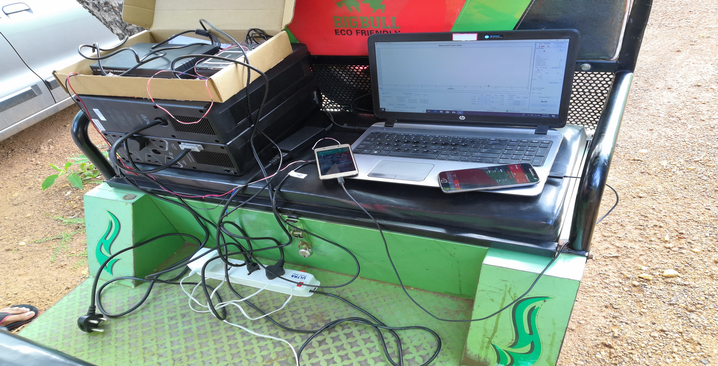
\includegraphics[width=0.31\textwidth]{img/pilot/setup}}%
	\hspace{0.1cm}
	\subfloat[Sorted throughput across the twenty-nine stretches of Fig.~\ref{fig:technology_with_traj} and the corresponding variations with RSSI, and Vertical and Horizontal Handovers]{%
		\label{fig:thptHO}%
		\fbox{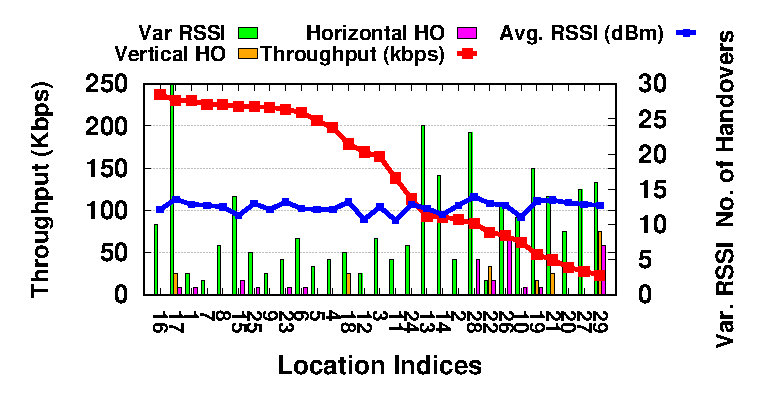
\includegraphics[width=0.31\textwidth]{img/pilot/location_throughput}}}%
	\hspace{0.1cm}
	\subfloat[Variations of Power Consumption with RSSI, and Vertical and Horizontal Handovers over the user's trajectory shown in Fig.~\ref{fig:technology_with_traj}]{%
		\label{fig:powerHO}%
		\fbox{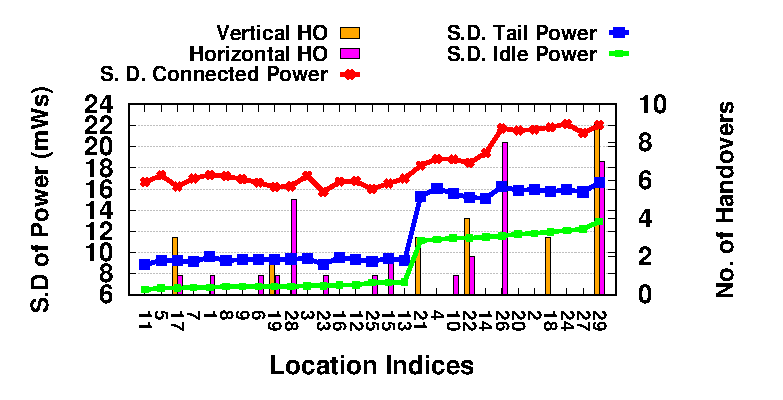
\includegraphics[width=0.31\textwidth]{img/pilot/location_power}}}
	\caption{Experimental setup and Throughput and Power consumption variations of a user under mobility; Phone: Moto G5, Service Provider: Airtel}\vspace*{-0.5cm}
\end{figure*}

\subsection{Deployability of the ABR algorithms}
In the recent years, there are lot developments in the area to adaptive bitrate algorithms. Some of those algorithms are based on different machine learning techniques like Penseive, HotDASH. These algorithms need powerful system to run and most of the algorithms have several library dependency which might not available is all the platform, specially smartphone and browsers. Most of the time it also need a trained model to get the optimal performance. As DASH like system uses a dumb server server and smart client, the algorithm need to be run in the client or the player it self. However, it is not feasible to run ML based ABR algorithm in the end user devices. 

Authors of this paper sometime provides a demo to run those algorithm in browser, but that technique is not scalable. For example authors of the pensieve run a ABR server in the client system and connect them from browsers javascript. It works, but it does not scale as every one need to run a local server. To overcome this problem we have developed a streaming system called Split-DASH. We discuss this architecture in details in section \ref{sec:Split_DASH_architecture}. 


 
%Although these algorithms have partially solved the problem and improved the quality of experience, these algorithms does provide the best quality of experience for users with mobility, especially in the developing country like India.

%Although 4G cellular network is deployed almost every corner of the country, it is not uniform. A smart phone need to fallback to 3G or 2G network. 

%Most of the video streaming provider uses streaming over HTTP. There are different streaming technology developed by different organization for example MPEG-DASH by DASHIF, smooth streaming by Adobe, HLS by Apple. These techniques are almost same even though these are developed independently. It 